\chapter{Statistical Machine Translation}
\label{chap:smt}

% TODO if time, add more hiero rule types, e.g. oov, deletions, etc.
% TODO if time, expand the hiero rule extraction section with the actual implementation
% TODO review all equations and make sure preceded by colon rather than period.
%TODO(remove "and colleagues")
%TODO add some related work for reparameterization of model 2 and maybe discriminative
%alignment ?
%TODO remove vertical bar for conditional proba
%TODO replace \ by \, in multiplications
%TODO replace all {\em
% TODO remove all \bf and \it and \bfseries and \itshape
% replace all refs by autoref
% TODO put a tilda before all citep
%TODO grep for trailing spaces
% TODO add a note in the extraction from posterior chapter that we use
% word-to-word HMM phrase posteriors as opposed to word-to-phrase HMM phrase
% posteriors
% TODO source channel or noisy channel model ?
% TODO Bill quick question: in MTTK f2e directory, what direction is it ?
% TODO for phrase pair extraction, cite also IEEE paper, not just Yonggang thesis
% TODO: papers to read: chen and goodman, yonggang IEEE, koehn's book
% TODO: see alternative presentation of rule extraction in one my reading group
% presentations
% TODO replace all refs by autoref
% TODO replace all HMMs by mbox{HMM}
% TODO remove all mbox and replace by text
% TODO maybe cite Yee Whye Teh's 2006 paper for lm
% TODO soften down claim that koehn et al is wrong in extraction from posteriors (which contradicts etc.)
% TODO maybe include alignment template paper
% TODO read papers by Papineni et al 1997, Papineni et al 1998
% TODO check instance of noisy channel and source channel
% TODO maybe include mention of Berger et al. 1994 The Candide System
% TODO look at this paper by Venugopal et al 2003: Effective Phrase Translation Extraction from Alignment Models
% TODO look at this paper: Papineni, Roukos, and Ward (1997, 1998)
% TODO look at this paper: Comparing and Integrating Alignment Template and Standard Phrase-Based Statistical Machine Translation
% TODO look at Knight 1999 that MT search is NP-complete
% TODO learn about A* search
% TODO learn about (admissible) heuristics used in phrase-based MT
% TODO review Zens et al 2002 KI 2002
% TODO maybe look at ngram translation models
% TODO note on how hiero models reordering directly but still can be improved
% a usual lexicalized reordering model
% TODO comment on hypothesis recombination and how a hyp may be lost for rescoring
% TODO maybe look at Tillmann et al 1997 for stack decoding
% TODO maybe look at A* search Och et al 2001
% TODO make a section with definitions
% TODO read the mathematics of SMT bordel de merde
% TODO grep for hyphen (phrase-based etc.)
% TODO harmonize notation \bm{f} vs. f_1^J
% TODO grep for cite grep -v citep or citet
% TODO grep for noindent
% TODO grep for {\em}, grep for {\bf}
% TODO grep for mbox
% TODO grep for linebreak


% This is a background chapter on SMT with emphasis on the parts
% that will be extended further for research.

%1st year report:
%-- definition hiero grammar
%-- rule patterns
%-- generative model, log linear model
%-- features
%-- metrics
%-- mert
%-- language modelling
%-- word alignment: hmm , ctext hmm, w2p hmm, symmetrisation
%-- rule extraction
%-- decoding with wfst
%-- rescoring

%currently:
%-- generative model
%-- word alignment: hmm, w2p hmm, symmetrisation
%-- language modelling
%-- phrase-based translation
%-- mert
%-- rescoring

%missing:
%-- mapreduce

%todo refs to background in other chapters:
%-- rule extraction alignment constraints
%-- wphmm
%-- lexical feature formula
%-- patterns and pattern filtering
%-- HiFST
%-- standard hiero grammar (patterns, etc.)
%-- mapreduce
%-- extraction constraints (retrieval and extraction)
%-- notation in background harmonized with the rest of chapters
%-- filters for grammar retrieval

%original source channel formulation OK
%word alignment OK
%newer log-linear formulation OK
%phrase-based translation NEW TODO
%hierarchical phrase-based translation OK
%features OK
%language modelling: one of the features OK
%optimization: metrics, mert OK
%hifst OK
%rescoring OK

%missing: mapreduce, phrase based translation

%\section{Overview}

% This should be an overview of the translation pipeline.
% TODO Maybe move it later as a summary and explanation of how things
% are done in practice

Statistical machine
translation (SMT)~\citep{lopez:2008:ACMComputingSurveys,koehn:2010:book}
has become the dominant approach to machine translation, as increasing
amounts of data and computing power have become available.
In the SMT paradigm, given a sentence in a source language, all
possible sentences in a target language are assigned a probability, a
score or a cost and the best translation is picked according to a certain
decision criterion that relates to these probabilities, scores or costs.

In this chapter, we first review the historical background of SMT in
\autoref{sec:historicalBackground}.
We then present the original source-channel model for SMT
in \autoref{sec:sourceChannelModel}.
Word alignment models, which we review in
\autoref{sec:StatisticalMachineTranslationWordAlignment},
were introduced within the framework of the source-channel
model. The original source-channel model was extended into the log-linear
model, presented in \autoref{sec:loglinearModel}.
The field of SMT shifted from word based models to phrase based
models, introduced in \autoref{sec:phraseBasedTranslation}, while
retaining word based models as a preliminary step. Hierarchical
phrase based translation, presented in
\autoref{sec:hierarchicalPhraseBasedTranslation}, is an extension
of phrase based translation that models gappy phrases and reordering
with a probabilistic synchronous context-free grammar. We then
examine various features employed in state-of-the-art decoders in
\autoref{sec:features}. The language model feature is explored in
more details in \autoref{sec:languageModelling}. In
\autoref{sec:optimization}, we review optimization techniques that
are employed in order to tune the feature weights. We finally present
how finite state transducers can be taken advantage of in decoding
in \autoref{sec:hifst} and rescoring in \autoref{sec:rescoring}.

\section{Historical Background}
\label{sec:historicalBackground}

%\begin{itemize}
%  \item warren weaver and the Translation report
%  \item development of rule based systems
%  \item development of word based systems + source channel model
%  \item development of phrase based systems + discr model
%  \item development of syntactic systems
%  \item neural networks ????
%\end{itemize}

%warren weaver
%historical survey: From First Conception to First Demonstration: the Nascent Years of Machine Translation, 1947–1954. A Chronology
%emphasize that the initial idea at a time when the idea is possible to implement dates from warren weaver. before that, just speculation since computers did not exist.
%talk about resurgence in mt of interlingua methods (tomas mikolov and word2vec software)
%mention quicksort as application of MT ?
%warren weaver Translation report: word 2 word translation not good. multiple meaning solution: look at context
%translation and cryptography a book written in Chinese is simply a book written in English which was coded into the the "Chinese code".
%translate with a certain confidence.
%language invariants: machine translation pyramid, interlingua, shout from building to building or go through the tunnel

In this section, we present a brief historical background of \emph{statistical}
machine translation. A more comprehensive account of the history
of machine translation in general can be found
elsewhere, e.g.~\citep{hutchins:1997:MT,hutchins:2000:MT}.

Warren Weaver can be considered the father of modern SMT.
At a time when the first computers are being developed, he
examines their potential application to the problem of machine
translation. In his memorandum~\citep{weaver:1955:Translation}, he
addresses the problem of multiple meanings of a source word
by considering the context of that source word, which heralds
phrase based translation techniques. He is also
the first to frame machine translation as a source channel
model by considering that a sentence in a foreign language
is some form of code that needs to be broken, in analogy
to the field of cryptography. He also emphasizes the
statistical aspect of machine translation. However, he also
predicts that the most successful approaches to machine
translation will take advantage of language invariants by
using an intermediate language representation in the translation
process. Even though state-of-the-art translation system do not
use this kind of approach, we do notice a resurgence in intermediate
language representation techniques~\citep{mikolov-le-sutskever:2013:arxiv}.

The first successful implementations of Warren Weaver's ideas
were carried out by IBM in the 1990s. The source channel
model together with a series of word alignment models were introduced
by~\citet{brown-dellapietra-dellapietra-mercer-1993} while
\citet{berger-dellapietra-dellapietra:1996:CL} addressed the problem
of multiple meanings using context in a maximum entropy framework.
Word-based models were extended into different variants
of phrase-based models at the
beginning of the century~\citep{koehn-och-marcu:2003:NAACL,och-ney:2004:CL}
and later on into hierarchical phrase-based models~\citep{chiang:2007:CL}.

\section{Source Channel Model}
\label{sec:sourceChannelModel}
% TODO check whether we say noisy channel or source channel model
% TODO normalize SMT
%brown et al series of papers directly inspired by warren weaver

%additional papers:
%brown et al 90: a statistical approach to machine translation


%notes for: a statistical approach to language translation
%glossary creation
%in the intro, phrase-based translation is basically described !!! partition source text into set of fixed locution (~ phrase), use glossary + contextual info to translate
%the phrases, arrange words in the target !!!!!!!!!!!!!!!!!!!!!!!!!!
%find word pairs using maximum mutual information criterion

(TODO Bill: do you say ``source channel model'' or ``noisy channel model'' ?)
Statistical machine translation was originally framed as a source channel
model~\citep{shannon:1948:BellSystemTechnicalJournal,brown-cocke-dellapietra-dellapietra-jelinek-lafferty-mercer-roossin:1990:CL,brown-dellapietra-dellapietra-mercer-1993}.
Given a
foreign sentence $\bm{f}$, we want to find the original English sentence
$\bm{e}$ that went through a noisy channel and produced $\bm{f}$. Note that in
the source channel model, what we would like to recover--the English sentence--is
called the \emph{source} while what is observed--the foreign sentence-- is
called the \emph{target}. We do not use this convention here and call the
\emph{source} what we are translated from and the \emph{target} what we are
translating into. We use the
decision rule in \autoref{eq:noisy}, which minimises the risk under a zero-one
loss function:
%
\begin{align}
  \hat{\bm{e}} &= \argmax_{\bm{e}} p(\bm{e} \mid \bm{f}) \nonumber \\
                &= \argmax_{\bm{e}} \frac{p(\bm{f} \mid \bm{e}) \, p(\bm{e})}{p(\bm{f})} \mbox{ (Bayes' rule)} \nonumber \\
                &= \argmax_{\bm{e}} p(\bm{f} \mid \bm{e}) \, p(\bm{e}) \label{eq:noisy}
\end{align}
%
$p(\bm{f} \mid \bm{e})$ is called the \emph{translation model} while
$p(\bm{e})$ is called the \emph{language model}. If $p(\bm{e} \mid \bm{f})$,
$p(\bm{f} \mid \bm{e})$ and $p(\bm{e})$ were perfectly estimated, the Bayes'
rule transformation would not be required and there would be no difference
between estimating a translation model only or both a
translation model and a language model. However, this is not the case as there
is a limited amount of data to train these models. In addition, the amount of
parallel data used to train the translation model is in general orders of
magnitude smaller than the
amount of monolingual data used to train the language model. It is therefore
preferable to train both a translation model and a language model.

We will see in the next section how the source channel model
can be used as a preliminary step in order to introduce
various word alignment models, by introducing word
alignment as a latent variable.

\section{Word Alignment}
\label{sec:StatisticalMachineTranslationWordAlignment}

In the previous section, we have described the source channel model, which
describes the translation process. This model cannot be used in
practice as it has too many parameters, namely all imaginable
sentence pairs. To address this issue,
\citet{brown-dellapietra-dellapietra-mercer-1993} introduce
the alignment between source words and target words as
a latent variable in the source channel model.

Given a sentence pair $(\bm{f}, \bm{e})$ with source sentence
length $J$ and target sentence length $I$, a word alignment $\bm{a}$
for this sentence pair is a mapping between the source and target
words. In other words, $\bm{a}$ is a subset of the cross product
of the set of source words and their positions and the set of target
words and their positions, as defined in \autoref{eq:alignmentSetDefinition}:
%
\begin{equation}
  \bm{a} \subset \{((f_j, j), (e_i, i)), (j, i) \in [1, J] \times [1, I]\}
  \label{eq:alignmentSetDefinition}
\end{equation}
%
Each element of $\bm{a}$ is called an \emph{alignment link}.
Alignment links between source and target words
correspond to semantic or syntactic equivalences shared by these words in the
source and target language. Alignments can present many-to-one and one-to-many
mappings as well as reordering as highlighted by crossing links. An example
of word alignment is
shown in Figure \ref{fig:examplealign}.
% TODO maybe add circles around the words
%
\begin{figure}
  \begin{center}
  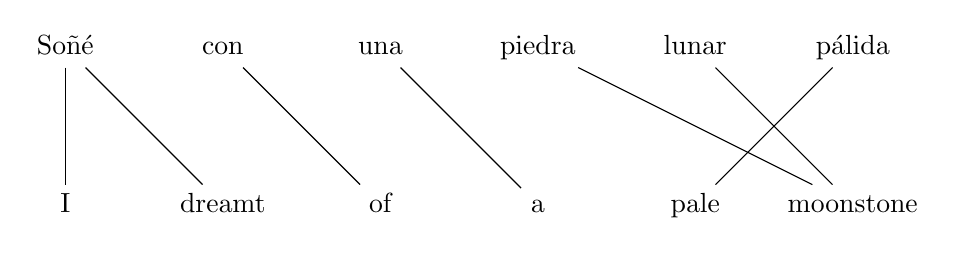
\begin{tikzpicture} [node distance = 2cm, text height=1.5ex, text depth=.25ex]
    % place nodes
    \node (Sone) {Soñé};
    \node [right of = Sone] (con) {con};
    \node [right of = con] (una) {una};
    \node [right of = una] (piedra) {piedra};
    \node [right of = piedra] (lunar) {lunar};
    \node [right of = lunar] (palida) {pálida};
    \node [below of = Sone] (I) {I};
    \node [right of = I] (dreamt) {dreamt};
    \node [right of = dreamt] (of) {of};
    \node [right of = of] (a) {a};
    \node [right of = a] (pale) {pale};
    \node [right of = pale] (moonstone) {moonstone};
    % draw edges
    \draw (Sone) -- (I);
    \draw (Sone) -- (dreamt);
    \draw (con) -- (of);
    \draw (una) -- (a);
    \draw (piedra) -- (moonstone);
    \draw (lunar) -- (moonstone);
    \draw (palida) -- (pale);
  \end{tikzpicture}
  \end{center}
  \caption{Example of word alignment for a Spanish-English sentence pair.}
  \label{fig:examplealign}
\end{figure}
%
\citet{brown-dellapietra-dellapietra-mercer-1993} introduce the
alignment $\bm{a}$ as a latent variable in the translation model
$p(\bm{f} \mid \bm{e})$, as in \autoref{eq:introduceAlignment}:
\begin{equation}
  p(\bm{f} \mid \bm{e}) = \sum_{\bm{a}} p(\bm{f}, \bm{a} \mid \bm{e})
  \label{eq:introduceAlignment}
\end{equation}
%
We abuse notation by calling $\bm{a}$ both the latent variable
and the set of alignment links, which is an instance of the latent
variable.
For mathematical convenience and in order to allow simplifications,
$\bm{a}$ is restricted to be a function from source word positions
to target word positions, as in \autoref{eq:alignmentDefinition}:
%
\begin{equation}
\begin{split}
  \bm{a} : [1, J] &\longrightarrow [0, I] \\
                j &\longmapsto a_j
\end{split}
\label{eq:alignmentDefinition}
\end{equation}
%
The target position zero is included to
model source words not aligned to any target word; these unaligned source words
are virtually aligned to a so-called \emph{null word}. Note that this definition
is not symmetric: it only allows many-to-one mapping from source to target.
Various symmetrisation strategies, presented in \autoref{sec:symmetrisationHeuristics},
have been devised to remedy this limitation. We can use the latent variable
$\bm{a}$ to rewrite the translation model in
\autoref{eq:generalEquationIBMModels}, with $\bm{f} = f_1^J$, $\bm{e} = e_1^I$
and $\bm{a} = a_1^J$:
%
\begin{equation}
  \begin{split}
    p(f_1^J \mid e_1^I) &= \sum_{a_1^J} p(f_1^J, a_1^J \mid e_1^I) \\
                        &= \sum_{a_1^J} \prod_{j = 1}^J p(f_j, a_j \mid f_1^{j - 1}, a_1^{j - 1}, e_1^I) \\
                        &= \sum_{a_1^J} \prod_{j = 1}^J p(f_j \mid f_1^{j - 1}, a_1^j, e_1^I) \, p(a_j \mid f_1^{j - 1}, a_1^{j - 1}, e_1^I) \\
  \end{split}
  \label{eq:generalEquationIBMModels}
\end{equation}
%
\citet{brown-dellapietra-dellapietra-mercer-1993} present a series
of five translation models of increasing complexity that parameterise the terms
$p(f_j \mid f_1^{j - 1}, a_1^j, e_1^I)$ and
$p(a_j \mid f_1^{j-1}, a_1^{j-1}, e_1^I)$.
Parameter estimation is carried out with the
expectation-maximisation algorithm~\citep{dempster-laird-rubin:1977:JRSS}.
Also based on \autoref{eq:generalEquationIBMModels}, \citet{vogel-ney-tillmann}
introduce an HMM model for word alignment and \citet{deng-and-byrne:2008:ASLP}
extend it to a word-to-phrase HMM model. We describe these two models in the following
sections.
% TODO should I present all IBM models ???

\subsection{HMM and Word-to-phrase Alignment Models}
\label{sec:statisticalMachineTranslationHmmAlignmentModel}

%TODO expand this section
\citet{vogel-ney-tillmann} introduce an HMM alignment model
that treats target word positions as hidden states and source words as
observations. The model is written in \eqref{eq:HmmAlignmentDefinition}:
%
\begin{equation}
  p(f_1^J, a_1^J \mid e_1^I) = \prod_{j=1}^J p(a_j \mid a_{j-1},I) \, p(f_j \mid e_{a_j})
  \label{eq:HmmAlignmentDefinition}
\end{equation}
%
Word-to-phrase HMM models~\citep{deng-and-byrne:2008:ASLP} were designed to
capture interesting properties of IBM Model
4~\citep{brown-dellapietra-dellapietra-mercer-1993} in an HMM framework in order
to keep alignment and estimation procedures exact. \autoref{fig:wordtophrase}
shows a simplified version of the generative story for an HMM word-to-phrase
alignment model: first, pick the number of target phrases $K$ according to
$P(K \mid I,J)$ where $I$ is the target length and $J$ the source
length\footnote{Again our source and target notation is inverted with respect
to the original publication: source denotes the language we translate from and
target the language we translate into}; then
pick a target word given the previously chosen one; finally generate the target
phrase from the source word using either unigram or bigram probabilities.
%
\begin{figure}
  \begin{center}
    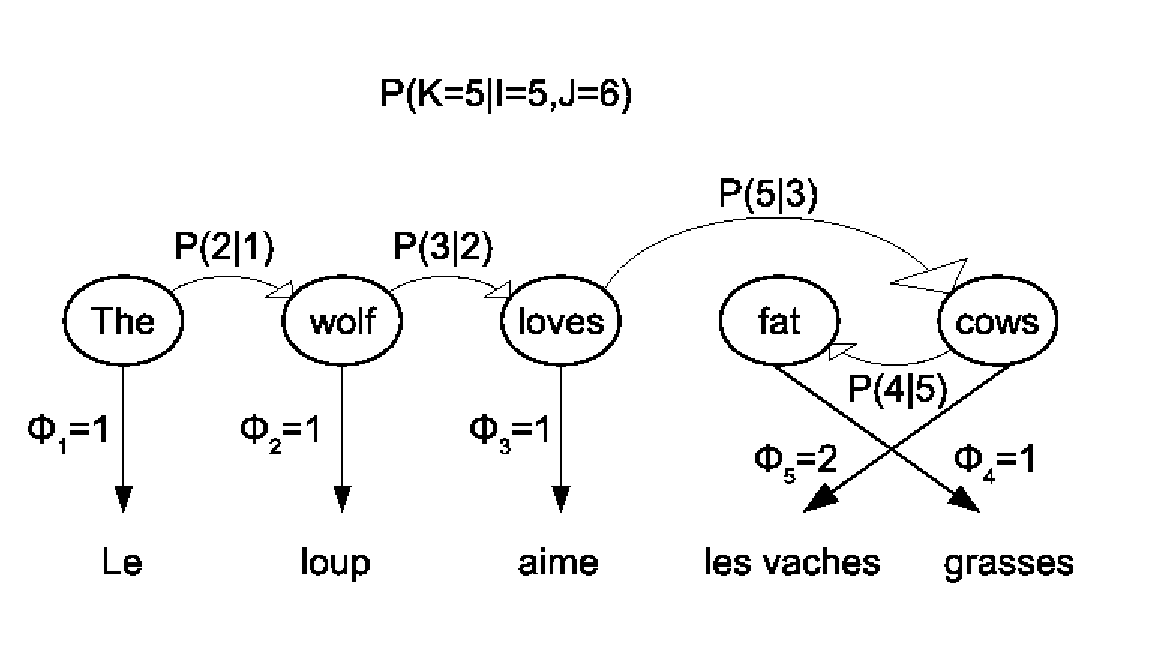
\includegraphics[scale=0.5]{figures/wordtophrase2.eps}
  \end{center}
  \caption{Illustrative example of an HMM word-to-phrase alignment model. The adjective noun sequence ``fat cows'' is
    reordered into the noun adjective sequence ``vaches grasses''. The word ``cows'' has fertility 2 as it is translated
    into the target phrase ``les vaches''.}
  \label{fig:wordtophrase}
\end{figure}
%
For example, if we use unigram probabilities, then we generate ``les vaches''
from ``cows'' according to
$P(\mbox{les vaches} \mid \mbox{cows}) = P(\mbox{les} \mid \mbox{cows}) P(\mbox{vaches} \mid \mbox{cows})$.
If we use bigram probabilities, then we generate ``les vaches'' from ``cows''
according to {\small $P(\mbox{les vaches} \mid \mbox{cows}) = P(\mbox{les} \mid \mbox{cows}) P(\mbox{vaches} \mid \mbox{cows},\mbox{les})$}.
Thus bigram probabilities take into account the context of the target word to
some extent.

\section{Log-Linear Model of Machine Translation}
\label{sec:loglinearModel}

%notes on adam berger paper
%model conditional prob
%p(y | x): x is phrase containing word "in", y is translation of "in"
%collect stats ptilda(x, y)
%binary feature: f(x, y) = 1 if y = en and April follows in
%expected value of f: ptilda(f) = sum_x,y ptilda(x,y) f(x,y)
%p(f) = sum_x,y ptilda(x) p(y | x) f(x,y)
%constraint: p(f) = ptilda(f)
%max entropy principle: choose p that satisfies the constraints
%and that maximizes entropy
%H(p) = -sum_x,y ptilda(x) p(y|x) log p(y|x)
%use Lagrange multiplier and Kuhn Tucker theorem to find that the solution
%is p(y|x) propto exp(\sum lambda_i f_i(x,y)). find lambda by max dual problem.
%also: p that satisfies constr and max entropy is also the
%p in the parametric family ... that maximizes likelihood of training sample.
%application to Candide.
%use max entropy modelling to predict translation of word in context.
%use max entropy modelling to predict word order.
%use max entropy modelling to segment.
%context dependent translation:
%first viterbi align training. then create events (x,y) (6 words
%surrounding in)
%incorporate this context dep translation into general translation model.

As we have seen in \autoref{sec:sourceChannelModel}, SMT was historically
framed as a source channel model.
\cite{berger-dellapietra-dellapietra:1996:CL} introduce maximum entropy
models for natural language processing. They show how a maximum entropy
model can be parameterized as an exponential, or log-linear model. They
apply this model to three machine translation related task. First, they
use a maximum entropy model to predict the translation of a word using
the context for that word. Then, they use a maximum entropy model to
predict the target language word order. Finally, they apply maximum
entropy modelling in order to predict the source sentence segmentation.

%notes och and ney 2002
%search done by the maximum approximation
%first present log linear model
%log linear model generalization of source channel model
%log linear model presented with additional alignment variable
%p(e_1^I, a_1^J | f_1^J) propto exp(sum_1^M lambda_m h_m(e_1^I, f_1^J, a_1^J))
%alignment template model
%p(f_1^J | e_1^I) = sum_{z_1^K, a_1^K} p(a_1^K | e_1^I) . p(z_1^K | a_1^K, e_1^I) . p(f_1^J | z_1^K, a_1^K, e_1^I)
%each component modeled with max entropy model

\citet{och-tillmann-ney:1999:EMNLP} notice that using an erroneous
version of the source channel model, that is using the following equation:
%
\begin{equation}
  \hat{\bm{e}} = \argmax_{\bm{e}} p(\bm{e} \mid \bm{f}) p(\bm{e})
\end{equation}
%
give comparable performance with respect to using the correct
formulation of the source channel model given in \autoref{eq:noisy}. In addition, it
allows them to use a dynamic programming algorithm for decoding.
\citet{och-ney:2002:ACL} propose the following extension:
%
\begin{align}
  \hat{\bm{e}} &= \argmax_{\bm{e}} p(\bm{e} \mid \bm{f}) \nonumber \\
               &= \argmax_{\bm{e}} \frac{\exp(\sum_{m=1}^M \lambda_m h_m(\bm{e}, \bm{f}))}{\sum_{\bm{e'}}\exp(\sum_{m=1}^M \lambda_m h_m(\bm{e'}, \bm{f}))} \nonumber \\
               &= \argmax_{\bm{e}} \exp(\sum_{m=1}^M \lambda_m h_m(\bm{e}, \bm{f})) \label{eq:loglinearModel}
\end{align}
%
where $h_m$ are called \emph{feature functions} and $\lambda_m$
are called \emph{feature weights}. The log-linear model is an extension
to the noisy channel model because it can be reduced to the original
noisy channel model with the following settings:
%
    \begin{itemize}
      \item $M = 2$
      \item $h_1({\bf e}, {\bf f}) = \log (p({\bf f}|{\bf e}))$
      \item $h_2({\bf e}, {\bf f}) = \log (p({\bf e}))$
      \item $\lambda_1 = \lambda_2 = 1$
    \end{itemize}
%
Log-linear models were originally trained with the maximum likelihood
criterion, which precisely makes them equivalent to maximum entropy
models~\citep{berger-dellapietra-dellapietra:1996:CL}. However,
more effective training techniques such as minimum error
training~\citep{och:2003:ACL} were introduced later on, that do
not require the computation of the normalization constant.
Thus, SMT are effectively simply linear models, with the objective
function presented in \autoref{eq:linearModel}:
%
\begin{equation}
  \hat{\bm{e}} = \argmax_{\bm{e}} \sum_{m=1}^M \lambda_m h_m(\bm{e}, \bm{f})
  \label{eq:linearModel}
\end{equation}

%In practice, \citet{och-ney:2002:ACL} do not use \autoref{eq:loglinearModel}.
%They introduce several latent variables in a so called \emph{alignment template}
%approach. The translation model is defined in \autoref{eq:alignmentTemplate}:
%
%\begin{equation}
%  p(e_1^I \mid f_1^J) = \sum_{z_1^K, a_1^K} p(a_1^K \mid e_1^I) p(z_1^K \mid a_1^K, e_1^I) p(f_1^J \mid z_1^K, a_1^K, e_1^I)
%  \label{eq:alignmentTemplate}
%\end{equation}
%
% TODO check if it is "correct" to invert the notation in above equation wrt to original publication
%where the variables $z_1^K$ and $a_1^K$ are alignment templates and the alignment of alignment templates.
%Each term in \autoref{eq:alignmentTemplate} is modelled as a maximum entropy model and search
%is carried out using the maximum approximation defined in \autoref{eq:maxApproximation}:
%
% TODO finish this
%\begin{align}
%  \hat{e_1^I} &= \argmax_{z_1}
%  \label{eq:maxApproximation}
%\end{align}

% TODO talk about training methods: GIS vs MERT

\section{Phrase Based Translation}
\label{sec:phraseBasedTranslation}

%notes on och et al 1999
%compare word based and phrase based
%e = argmax p(e) p(f|e)
%word based model: each source word (french) assigned exactly one target word (english)
%difficult to model context and also to translate compound words
%model two alignment levels: phrase level alignment between phrases and word level alignment between words within phrases
%word based approach: use an HMM
%p(f_1^J | e_1^I) = sum_{a_1^J} prod_j p(a_j | a_{j - 1}) p(f_j | e_{a_j})
%some restrictions are used (so called monotonicity): alignment jump between a_{j - 1} and a_j can only be 0, 1, 2.
%Q_{e'}(j, e): probability of best partial hypothesis (e_1^i, a_1^j) with e_i = e, e_{i - 1} = e' and a_j = i
%search: mapping j -> (a_j, e_{a_j})
%DP recursion:
%Q_e'(j, e) = p(f_j | e) . max {
%  p(0) . Q_e'(j - 1, e),
%  p(1) . max_e'' {p(e | e', e'') Q_e''(j - 1, e')},
%  p(2) . max_{e'', e'''} {p(e | e', e'') . p(e' | e'', e''') . Q_e'''(j - 1, e'')}
%  }
%optimal translation: max_e',e Q_e'(J, e) . p(\$ | e, e')
%extension to one-to-many alignment model.
%solution: reverse translation direction, then extend English vocab with multiple words, then redo standard training for original translation direction.
%alignment template approach
%problem with word based models: only allow one to many or many to one, or many to many but hacky solution
%model phrase to phrase is a way to model context.
%alignment template z: triple (Ftilda, Etilda, Atilda) alignment Atilda between source class sequence Ftilda and
%target class sequence Etilda.
%Atilda: matrix with binary values
%Atilda allows for many to many
%Ftilda and Etilda automatically trained bilingual classes
%use classes for better generalization
%alignment template applicable to sequence source words ftilda if
%alignment template classes and classes of source words are equal
%application of alignment template contraints the target words to have the right classes
%selection target words: p(etilda | z, ftilda)
%p(ftilda | (Ftilda, Etilda, Atilda), etilda) = delta(classes(etilda), Etilda) delta(classes(ftilda), Ftilda) prod_{j=1}^J (I???) p(f_j | Atilda, etilda)
%p(f_j | Atilda, etilda) = sum_{i = 0}^I p(i | j; Atilda) p(f_j | e_i)
%p(i | j, Atilda) = Atilda(i, j) / (sum_i Atilda(i, j))
%rien compris
%phrase level alignment
%decompose f_1^J and e_1^I into sequence of phrases
%f_1^J = ftilda_1^K
%assume that there is only one possible segmentation (possibly one of the differences between Och and Koehn)
%p(f_1^J | e_1^I) = p(ftilda_1^K | etilda_1^K)
%                 = sum_{atilda_1^K} p(atilda_1^K, ftilda_1^K | etilda_1^K)
%                 = sum_{atilda_1^K} p(atilda_1^K | etilda_1^K) p(ftilda_1^K | atilda_1^K, etilda_1^K)
%                 = sum_{atilda_1^K} prod_{k = 1}^K p(atilda_k | atilda_1^{k-1}, K) p(ftilda_k | etilda_{atilda_k})
%p(ftilda | etilda) = sum_z p(z| etilda) p(ftilda | z, etilda)
%training: s2t and t2s hmm without the max approximation
%get the viterbi alignments a_1^J and b_1^I
%use the grow diag symmetrisation heuristic.
%estimate bilingual word lexicon p(f|e): n_A(f, e) | n(e)
%train world classes
%extract consistent phrase pairs from alignment
%obtain n(z) of how often alignment template occurs in aligned corpus.
%relative freq estimate: p(z = (Ftilda, Etilda, Atilda) | etilda) = n(z) . delta(classes(etilda), Etilda) / n(classes(etilda))
%decoding search
%objective: argmax_{e_1^I} p(e_1^I p(e_1^I | f_1^J)) (wrong version of source channel model)
%use class-based 5g lm
%preprocessing before translation: filter alignment templates per source sentence, segment source sentence
%segmentation objective: argmax_{ftilda_1...ftilda_k = f_1^J} prod_{k=1}^K max_z p(z | ftilda_k)
%search: produce partial hypotheses with info: last target word, language model state,
%source coverage, last alignment template, position of last target word in alignment template
%instantiation (???), cost so far, backpointer
%integrate future cost because compare hypotheses that cover different parts of the input

%notes on och-ney 2004 (journal paper version of och et al. 1999)
%overview: align, extract, extracted phrases with alignment and word classes are
%called alignment templates
%log-linear model: hat{e_1^I} = argmax_{e_1^I} p(e_1^I | f_1^J)
%                             = argmax exp(sum_m=1^M lambda_m h_m(e_1^I, f_1^J))/Z
%parameters lambda trained with MLE (same as maximum entropy)
%or trained with MERT
%use latent variable
%p(e_1^I, a_1^J | f_1^J) = (1/Z) . exp(sum_1^M lambda_m h_m(e_1^I, f_1^J, a_1^J))
%description of word alignments etc.
%description of symmetrisation heuristics etc.
%symmetrized Viterbi alignments used to compute translation lexicon
%description of phrase-extract
%alignment templates: replace words with word classes and store
%alignment info for each phrase pair
%alignment template z = (F_1^J', E_1^I', Atilda)
%F_1^J' source class sequence
%E_1^I' target class sequence
%Atilda: alignment between source class seq and target class seq
%automatically train bilingual classes
%notation: etilda, ftilda target and source phrases
%p(z = (F_1^J', E_1^I', Atilda) | ftilda) = N(z) . delta(F_1^J', C(ftilda)) / N(C(ftilda%))
%remove alignment templates with prob less than 0.01
%limit on source phrase: between 4 and 7
%translation model
%f_1^J = ftilda_1^K
%e_1^I = etilda_1^K
%model described for a specific segmentation but in search
%optimal segmentation also searched for
%pi_1^K: permutation of the phrases, models phrase reordering
%etilda_k is translation of ftilda_{pi_k}
%alignment template between f_{pi_k} and e_k: z_k
%hidden variables in the model: pi_1^K, z_1^K
%use log-linear model, feature functions depend on source, target and hidden variables
%features
%alignment template selection
%h_AT(e_1^I, f_1^J, pi_1^K, z_1^K) = log prod_1^K p(z_k | f_{j_{pi_k - 1} + 1}^{j_{pi_k}%})
%h_WRD(e_1^I, f_1^J, pi_1^K, z_1^K) = log prod_1^I p(e_i | {f_j, (i,j) in A}, E_i)
%p(e_i | {f_j, (i,j) in A}, E_i)
%etc etc. hyper complique
%h_AL phrase alignment (reordering model)
%h_AL(e_1^I, f_1^J, pi_1^K, z_1^K) = sum_{k=1}^{K+1} |j_{pi_k - 1} - j_{pi_{k - 1}}
%3gram lm + 5g class based lm
%training: blabla
%search
%breadth-first search with pruning: beam search
%search objective:
%hat{e_1^I} = argmax_{e_1^I} sum_{pi_1^K, z_1^K} p(e_1^I, z_1^K, pi_1^K | f_1^J)
%           ~~ argmax_{e_1^I, pi_1^K, z_1^K} p(e_1^I, z_1^K, pi_1^K | f_1^J)
%           = argmax_{e_1^I, pi_1^K, z_1^K} sum_{m = 1}^M lambda_m h_m(e_1^I, f_1^J, pi_%1^K, z_1^K)
%use the max approximation
%structure of search space
%generate hypothesis left to right on the target
%preprocessing step: first determine all source phrases that match an alignment template
%unknown words carried over
%use 5-best target words for each target class according to some criterion
%use hypothesis recombination
%pruning done for hypotheses that cover the same number of source words
%future cost estimation
%rien compris
%exps etc. etc.

%notes on phrase-based mt by koehn's book
%EM training of phrase-based models: NO
%Extensions to the Reordering Model
%zh-en, ar-en, fr-en in contrast to de-en or jp-en
%lexicalized reordering
%reordering model p_o predicts orientation m,s,d given phrase pair f,e:
%p_o(orientation | f, e)
%extract each phrase pair with orientation type p_o(orientation | f, e) = count(orientation, e, f) / sum_o count(o, e, f)
%to be smoothed with prior p_o(orientation)
%phrase translation as classification: use max ent model to model context
%use phrase penalty to model source segmentation
%use word penalty to model length
%lexical weighting a la koehn
%used as smoothing for translation model
%lex(e|f, a) = prod_{i = 1}^length(e) (1/|{j | (i,j) in a}|) sum_{j | (i,j) in a} w(e_i | f_j)
%if english word unaligned, use the NULL word on the f side
%w estimated with rel freq from aligned corpus.
%use both lex(e|f,a) and lex(f|e,a)
%log linear model: TODO find out what's the objective in moses/koehn2003
%phrase-extract etc. etc.
%source channel phrase-based model:
%e = argmax p(f|e) p(e)
%  = argmax prod_i p(f_i | e_i) d(start_i - end_{i - 1} -1)
%justification: segmentations are equally likely, max approximation ??
%d(x) propto alpha^|x|

%notes on phrase-based mt decoding by koehn's book
%description of hypothesis expansion
%computational complexity: NP complete/hard
%hypothesis recombination
%simple example: [it] [is] vs. [it is]
%more complicated example: [he] [does not] vs. [it] [does not]
%note: instead of deleting the hyp, we still keep pointer
%so that we can output n-best
%stack decoding
%stack <-> number of foreign words translated
%problem: some hyps in a stack cover different regions of the input
%histogram pruning and threshold pruning
%reordering limit in search
%future cost or outside cost or rest cost
%cost of translation option: translation cost easy,
%language model cost approximated by lm without context,
%reordering model ignored
%for each translation option, compute the ``cost without context''
%then estimate the cheapest cost for translating any span in the
%input using DP
%use future cost in search: add the cost of the remaining (gappy) span
%to the partial cost

%notes on koehn et al 2003
%"Note that phrase translation with a lexical weight is a
%special case of the alignment template model [Och et al.,
%1999] with one word class for each word."

So far, we have presented two modelling approach to machine translation,
the original source channel model and the current log-linear model. We also
have presented word alignment, which was introduced in the source channel
model framework and which is a word based model.

% TODO motivation for phrase based: word based a:[1,J]->[1,I] so many to one mapping only
Phrase-based models were introduced as a practical solution to the
problem of translating words in context. Phrase-based models
currently achieve state-of-the-art performance. They can be defined
in the source channel model framework or the log-linear model framework.
Because the source channel model is rarely used anymore and because it is
a special case of a log-linear model, we will focus our presentation
on the log-linear model.

There are different variations on the phrase-based translation paradigm.
We will focus on two popular approaches, namely the alignment template
system~\citep{och-tillmann-ney:1999:EMNLP,och-ney:2004:CL} and the phrase-based
system~\citep{koehn-och-marcu:2003:NAACL,koehn:2010:book}.

\subsection{Alignment Template Phrase-Based Model}

The alignment template system uses a log-linear model presented
in \autoref{eq:loglinearModel} as a starting point and repeated in
\autoref{eq:loglinearModelRepeated}:
%
\begin{equation}
  \hat{\bm{e}} = \argmax_{e_1^J} \exp(\sum_{m = 1}^M \lambda_m h_m(f_1^J, e_1^I))
  \label{eq:loglinearModelRepeated}
\end{equation}
%
In order to reduce the number of parameters, the two latent variables $\pi_1^K$
and $z_1^K$ are introduced. $z_1^K$ is a sequence of \emph{alignment templates}
while $\pi_1^K$ is a permutation of size $K$. An alignment template
is a triple $(\tilde{F}, \tilde{E}, \tilde{A})$ where $\tilde{F}$ is a
sequence of source word classes, $\tilde{E}$ is a sequence of target
word classes and $\tilde{A}$ is an alignment between $\tilde{F}$
and $\tilde{E}$. $\pi_1^K$ together with $z_1^K$ define
a source segmentation of $f_1^J$ into source phrases $\tilde{f}_1^K$,
a target segmentation of $e_1^I$ into target phrases $\tilde{e}_1^K$ and
a bijective mapping between source phrases and target phrases where
$\tilde{f}_{\pi_k}$ is mapped to $\tilde{e}_{k}$ for $k \in [1,K]$.
The alignment templates $z_1^K$ are constrained in such a way that
the alignment template classes match the word classes.

Using the max approximation and making the feature
functions depend on the hidden variables, the translation model
can be rewritten in \autoref{eq:alignmentTemplateModel}:
%
\begin{equation}
  \hat{\bm{e}} = \argmax_{e_1^J, z_1^K, \pi_1^K} \exp(\sum_{m = 1}^M \lambda_m h_m(f_1^J, e_1^I, \pi_1^K, z_1^K))
  \label{eq:alignmentTemplateModel}
\end{equation}
%

\subsection{Standard Phrase-Based Model}

The standard phrase-based model is similar to the alignment template
model but does not make use of source and target word classes.
Again, we use the latent variables $\pi_1^K$ and $z_1^K$.
This time, $z_k$ is defined as a triple $(\tilde{f}, \tilde{e}, \tilde{A})$
where $\tilde{f}$ is a sequence of source words, $\tilde{e}$ is a sequence
of target words and $\tilde{A}$ is an alignment between $\tilde{f}$ and $\tilde{e}$.
The reason for using the alignment information between phrase pairs is to be able
to compute the lexical feature. Because the lexical feature can be computed
by other means than this alignment information, it is also possible to simply
define $z_k$ as a phrase pair.

We have presented two variants of the phrase-based model. We will now
describe how to obtain the phrase pairs used for the latent variable $z$.

\subsection{Symmetrisation Heuristics}
\label{sec:symmetrisationHeuristics}

A preliminary step to phrase pair extraction is to symmetrize alignments.
As noted in \autoref{sec:StatisticalMachineTranslationWordAlignment}, alignment
models are not symmetric as they only allow many-to-one mapping from source to
target. \citet{och-tillmann-ney:1999:EMNLP} designed
a heuristic to symmetrise alignments trained in both source to target
and target to source directions. \citet{koehn-och-marcu:2003:NAACL}
later extend the set of heuristics and examine the impact on translation
performance for each heuristic.

Let us consider a sentence pair $(\bm{f}, \bm{e})$,
an alignment
from $\bm{e}$ to $\bm{f}$, $\bm{a_{e2f}}$, and an alignment from $\bm{f}$ to
$\bm{e}$, $\bm{a_{f2e}}$. Different symmetrisation heuristics that result in a
symmetric alignment $\bm{a}$ are defined as follows:
%
\begin{itemize}
  \item \emph{Union}: $\bm{a} = \bm{a_{e2f}} \cup \bm{a_{f2e}}$
  \item \emph{Intersection}: $\bm{a} = \bm{a_{e2f}} \cap \bm{a_{f2e}}$
  \item \emph{Grow-diag} (grow diagonal): $\bm{a} = (\bm{a_{e2f}} \cap \bm{a_{f2e}}) \cup GD$. $GD$ is the set of
    alignment links that are in the union and not in the intersection, whose words are not already aligned and
    that are neighbours of alignment links in the intersection.
\end{itemize}
%
%Symmetrised alignments have be shown to produce better translation results than
%unidirectional alignments. However, we find in one of our experiments that this
%is not always the case (see \autoref{sec:extractionFromPosteriorsSymmetrising}).

% This should review phrase based SMT.
% Why: the gyro decoder is like a phrase based SMT decoder.

% phrase based extraction + stack base decoding

\subsection{Phrase Pair Extraction}
\label{sec:phrasextract}

Grammar rules are extracted from symmetrised alignments.
Let us consider a sentence pair $(\bm{f},\bm{e})$ and an alignment $\bm{a}$.
We extract all phrase pairs that are {\em consistent} with the alignment.
This means that we extract all phrase pairs $(f_{j_1}^{j_2},e_{i_1}^{i_2})$ that
satisfy \autoref{eq:consistent} and \autoref{eq:atLeastOneLink}:
%
\begin{align}
  & \forall (j,i) \in \bm{a}, (j \in [j_1, j_2] \Leftrightarrow i \in [i_1,i_2]) \label{eq:consistent} \\
  & [j_1, j_2] \times [i_1, i_2] \cap \bm{a} \neq \emptyset \label{eq:atLeastOneLink}
\end{align}
%
%TODO better example
\autoref{eq:consistent} requires that no alignment link be between a word
inside the phrase pair and a word outside the phrase pair.
\autoref{eq:atLeastOneLink} requires that there be at least one alignment link
between a source word in the source phrase and a target word in the target phrase.
For example, in Figure \ref{fig:ruleextract}, the phrase pair
(Buenas tardes, Good afternoon) is extracted while the
phrase pair (tardes !, !) is not because the word ``tardes'' is aligned
outside the phrase pair.
%
      \begin{figure}[h]
        \begin{center}
          \vspace*{-5cm}
          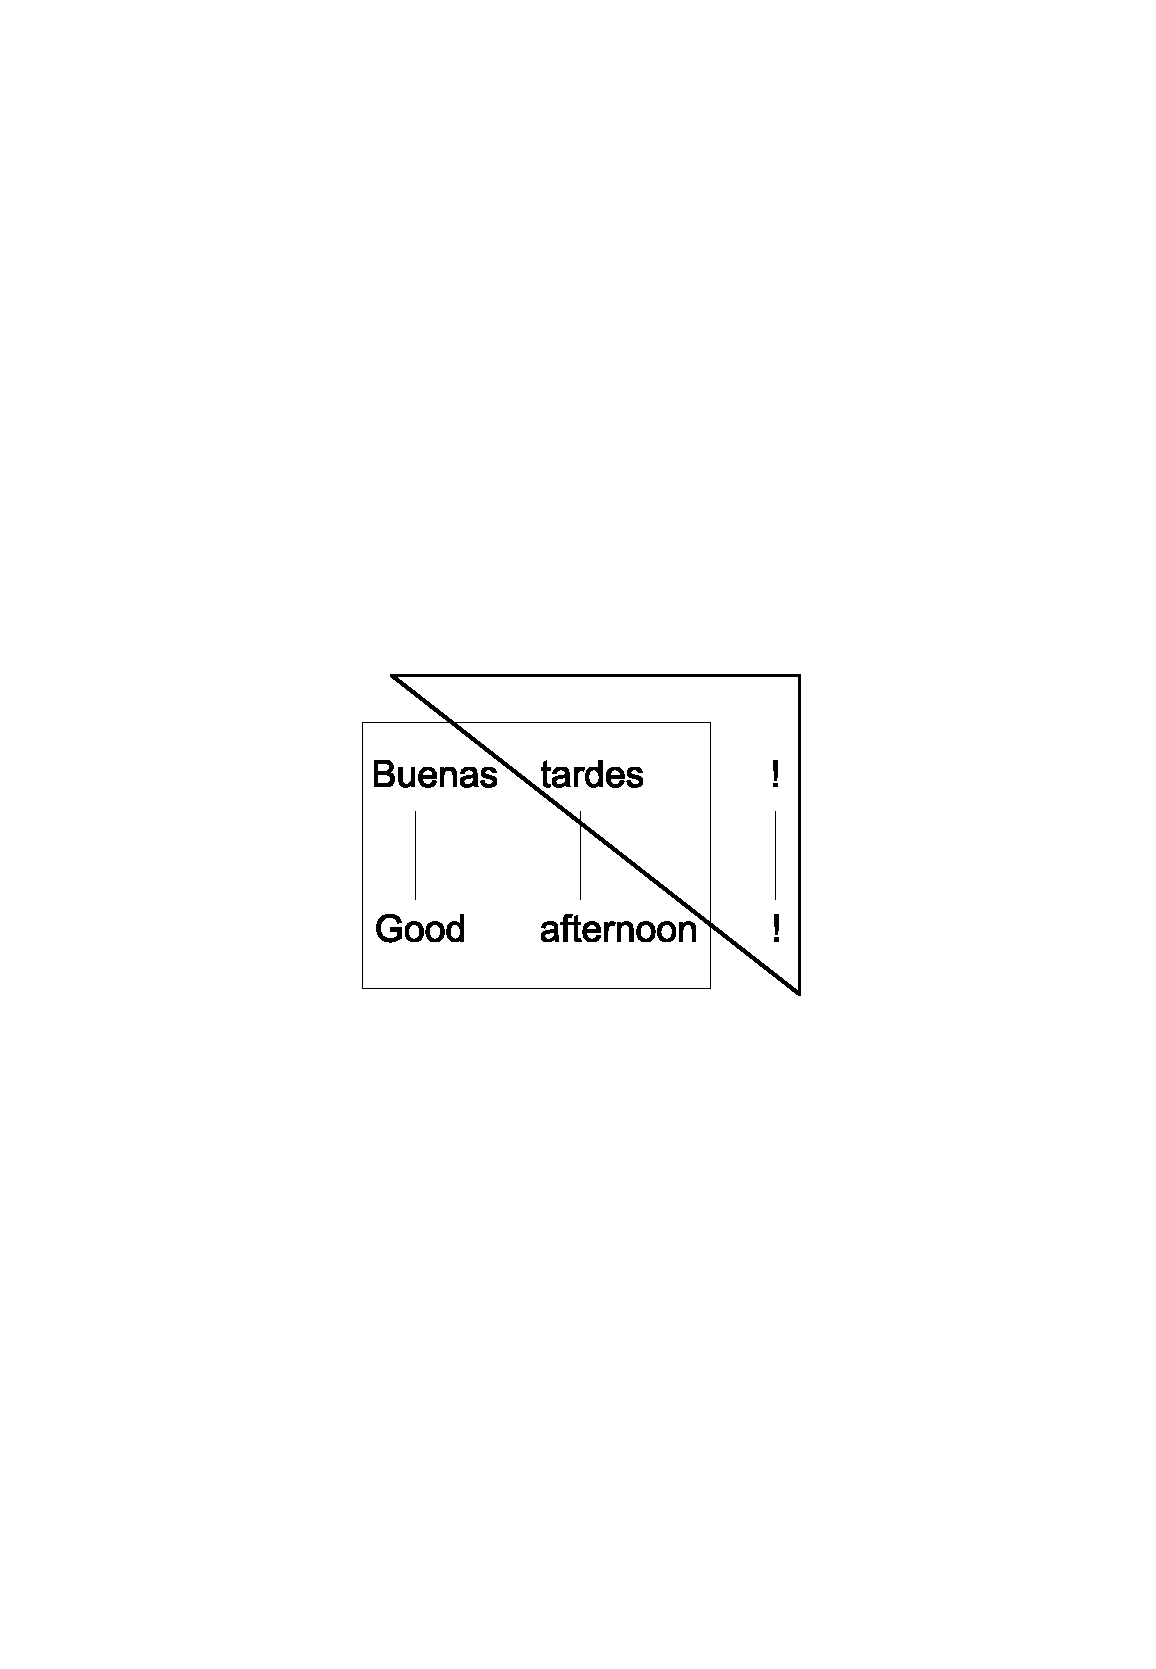
\includegraphics[scale=0.5]{figures/phraseextraction.eps}
          \vspace*{-5cm}
        \end{center}
        \caption{Rule extraction for a sentence pair. For example, the phrase (Good afternoon, Buenas tardes) is extracted. The phrase pair (tardes !, !) is not extracted because it is
        not consistent with the alignment.}
        \label{fig:ruleextract}
      \end{figure}

\subsection{Phrase Based Decoding}

%notes on knight 1999 NP complete
%blabla on cryptograph and pos tagging
%machine translation
%v total English words
%bigram source model with v^2 parameters
%substitution/permutation channel models
%parallel corpus (sentence length <= m)
%monolingual french (???) sentence (length <= m)
%e_i has fertility phi_i: parameter n(phi | e)
%french words produced according to s(f|e) and permuted according to d(j|i,m,l)
%model 1 EM training
%collect estimate epsilon(m | l) from data
%set s(f|e) uniform initially
%basically, decoding with M1 is NP-complete
%reduction from hamilton circuit

We can now present the decoding process in phrase based translation.
We will first introduce the translation process. Then, we will
describe how translation hypotheses are built incrementally.
We will then motivate the need for pruning and how pruning
is carried out. Finally, we will describe how future cost estimation
may reduce search errors.

\paragraph{Translation Process}

Given a source sentence, the translation process is to iteratively
pick a source phrase, translate that source phrase into a target phrase
and append the target phrase to the translation, until the source
sentence has been entirely covered by source phrases. While the process is not
complete, the concatenation of target phrases is called a
\emph{partial hypothesis}.

\paragraph{Hypothesis Expansion}

The decoding process starts from an initial empty partial hypothesis.
This empty partial hypothesis is extended by picking source phrases,
appending their translations to the empty hypothesis.
At this stage, we have obtained several partial hypotheses.
The partial hypotheses are repeatedly extended until
all source words have been covered.
Partial hypotheses are represented by states
that contain the information necessary to
compute the cost of an extension.
If we use an $n$-gram language model as a feature,
the state will encode the cost of the partial hypothesis
and the last $n - 1$ words of the partial hypothesis.

\paragraph{Hypothesis Recombination}

When two partial hypothesis share the same $n - 1$
words, only the partial hypothesis with the lower
cost can lead to the best final hypothesis. Therefore,
the partial hypothesis with higher cost can be discarded, or
alternatively, it is possible to make these two partial
hypotheses share the same state for rescoring purposes.

\paragraph{Stack Based Decoding and Pruning}

The decoding search space is very large: given a source sentence of size
$J$, the translation process has to pick one of $2^J$ possible segmentation
in order to obtain a source phrase sequence, then pick a permutation
for that source phrase sequence and finally pick a translation for each
phrase. Therefore, a decoder has to make approximations.

The partial hypotheses mentioned above are grouped in \emph{stacks}
by the number of source words covered.
This allows pruning. Each time a hypothesis expansion produces a hypothesis that
belongs to a certain stack, that stack is pruned.
There are two types of pruning, histogram pruning and threshold
pruning. Histogram pruning enforces a maximum number
of partial hypotheses in each stack. Threshold pruning
examines the cost of the best partial hypothesis in a stack
and discards all partial hypotheses in that stack whose cost
is greater than the best cost plus a threshold.

\paragraph{Future Cost}

Partial hypotheses that cover the same number of source
words are grouped together for pruning purposes. However,
their cost may not be directly comparable, for example
partial hypotheses that correspond to the translation of frequent
words in the source might have a smaller cost than partial hypotheses
that correspond to the translation of rare words in the source.
To address this issue, a future cost that represents how difficult it is
to translate the rest of the sentence is added to the model cost of each
partial hypothesis.

\section{Hierarchical Phrase-Based Translation}
\label{sec:hierarchicalPhraseBasedTranslation}

  \subsection{Introduction and Motivation} \label{sec:hierintro}

  Hierarchical phrase-based translation (hierarchical translation in short) was shown to
  outperform state-of-the-art phrase-based systems~\citep{chiang:2005:ACL,chiang:2007:CL}.
  Hierarchical translation relies on the hierarchical grammar formalism defined in Section \ref{sec:hiergrammar}. A closely related formalism, inversion
  transduction grammars, was previously introduced~\citep{wu:1995:IJCAI,wu:1997:CL}. The motivation for this type
  of formalism is to allow nested reordering which can happen between language pairs with very different word order such as 
  Chinese and English. For example, the Chinese sentence with English gloss in \autoref{fig:example} requires nested reordering~\citep{chiang:2007:CL}.


  \begin{figure}
    \begin{center}
      \begin{footnotesize}
      %\begin{tabular}{*{11}{l}}
      \begin{tabular}{p{0.9cm} p{1cm} p{0.2cm} p{0.3cm} p{1.9cm} p{0.3cm} p{1.5cm} p{0.3cm} p{0.9cm} p{1cm} p{0.9cm}}
%        \textbf{Chinese} & 澳洲 & 是 & 与 & 北韩 & 有 & 邦交 & 的 & 少数 & 国家 & 之一 \\
        \textbf{Pinyin}  & Aozhou & shi & yu & Beihan & you & bangjiao & de & shaoshu & guojia & zhiyi \\
        \textbf{Gloss} & Australia & is & with & North Korea & have & dipl. rel. & that & few & countries & one of \\
         & & & & & & & & & & \\
        \textbf{English} & \multicolumn{10}{l}{Australia is one of the few countries that have diplomatic relations with North Korea} \\
      \end{tabular}
      \end{footnotesize}
    \end{center}
    \caption{Example of Chinese sentence that needs nested reordering to be translated into English.}
    \label{fig:example}
  \end{figure}

  
%  \begin{figure}
%    \begin{center}
%      \includegraphics[width=13cm]{figures/example.ps}
%    \end{center}
%    \caption{Example of Chinese sentence with English gloss that needs nested reordering to be translated into English}
%    \label{fig:example}
%  \end{figure}
  

  \begin{itemize}
    \item ``with North Korea have diplomatic relations'' must be reordered into 
      ``have diplomatic relations with North Korea''.
    \item ``few countries one of'' must be reordered into ``one of (the) few countries''.
    \item After the two previous segments are reordered, ``have diplomatic relations with North Korea that one of the few countries'' must be reordered into ``one of the few countries that have diplomatic relations with North Korea''.
  \end{itemize}
%
  Phrase-based systems can model this type of movement but they need to use very long phrase pairs, which is
  impractical because of data sparsity. On the other hand, hierarchical grammars do model this type of movement using
  shorter phrase pairs.

  \subsection{Hierarchical Grammar} \label{sec:hiergrammar}

  A hierarchical grammar, which is a particular instance of a synchronous context free grammar is a set of rewrite rules of the following type:

  \begin{equation}
    X \rightarrow \langle \gamma, \alpha, \sim \rangle \nonumber
  \end{equation}

  \noindent where $X$ is a nonterminal, $\gamma$ and $\alpha$ are sequences of terminals and nonterminals and $\sim$ is an alignment
  between nonterminals. Terminals that appear in $\gamma$ are words in the source language while terminals that appear in $\alpha$ are
  words in the target language. Nonterminals are chosen from a finite set disjoint from the set of terminals. The alignment between nonterminals
  indicates which nonterminals in the source and target languages correspond to each other. The alignment $\sim$ can be written with 
  a set of matching indices.

  A hierarchical grammar also usually contains the following rules called glue rules:

  \begin{eqnarray}
    S &\rightarrow& \langle X, X \rangle \nonumber \\
    S &\rightarrow& \langle S X, S X \rangle \nonumber
  \end{eqnarray}

  \noindent with $S$ the start symbol. The first glue rule is necessary to be able to start a derivation.
  The second glue rule allows concatenation of phrases or rules.

  Let us consider for example the following grammar~\citep{chiang:2007:CL} where each rewrite rule is given a name $R_i$:

  \begin{eqnarray}
    R_1&:& S \rightarrow \langle X, X \rangle \nonumber \\
    R_2&:& S \rightarrow \langle S X, S X \rangle \nonumber \\
    R_3&:& X \rightarrow \langle X_1 \mbox{ de } X_2, \mbox{ the } X_2 \mbox{ that } X_1 \rangle \nonumber \\
    R_4&:& X \rightarrow \langle X \mbox{ zhiyi}, \mbox{ one of } X \rangle \nonumber \\
    R_5&:& X \rightarrow \langle \mbox{yu } X_1 \mbox{ you } X_2, \mbox{ have } X_2 \mbox{ with } X_1 \rangle \nonumber \\
    R_6&:& X \rightarrow \langle \mbox{Aozhou}, \mbox{ Australia} \rangle \nonumber \\
    R_7&:& X \rightarrow \langle \mbox{shi}, \mbox{ is} \rangle \nonumber \\
    R_8&:& X \rightarrow \langle \mbox{Beihan}, \mbox{ North Korea} \rangle \nonumber \\
    R_9&:& X \rightarrow \langle \mbox{bangjiao}, \mbox{ diplomatic relations} \rangle \nonumber \\
    R_{10}&:& X \rightarrow \langle \mbox{shaoshu guojia}, \mbox{ few countries} \rangle \nonumber
  \end{eqnarray}
%
  With this grammar, it is possible to write a derivation, that is a sequence of rules, that rewrites the start symbol $S$ into the sentence pair presented in Section \ref{sec:hierintro} \cite{chiang:2007:CL}. For example we can apply the derivation \linebreak $R_2,R_2,R_1,R_6,R_7,R_4,R_3,R_{10},R_5,R_9,R_8$ as
  follows:

  \begin{footnotesize}
  \begin{eqnarray}
    S &\rightarrow& \langle S X, S X \rangle \nonumber \\
      &\rightarrow& \langle S X_1 X_2, S X_1 X_2 \rangle \nonumber \\
      &\rightarrow& \langle X_1 X_2 X_3, X_1 X_2 X_3 \rangle \nonumber \\
      &\rightarrow& \langle \mbox{Aozhou } X_2 X_3, \mbox{Australia } X_2 X_3 \rangle \nonumber \\
      &\rightarrow& \langle \mbox{Aozhou shi } X_3, \mbox{Australia is } X_3 \rangle \nonumber \\
      &\rightarrow& \langle \mbox{Aozhou shi } X \mbox{ zhiyi}, \mbox{Australia is one of } X \rangle \nonumber \\
      &\rightarrow& \langle \mbox{Aozhou shi } X_1 \mbox{ de } X_2 \mbox{ zhiyi}, \mbox{Australia is one of the } X_2 \mbox{ that } X_1 \rangle \nonumber \\
      &\rightarrow& \langle \mbox{Aozhou shi } X_1 \mbox{ de shaoshu guojia zhiyi}, \mbox{Australia is one of the few countries that } X_1 \rangle \nonumber \\
      &\rightarrow& \langle \mbox{Aozhou shi yu } X_1 \mbox{ you } X_2 \mbox{ de shaoshu guojia zhiyi}, \nonumber \\
      &&                    \mbox{Australia is one of the few countries that have } X_2 \mbox{ with } X_1 \rangle \nonumber \\
      &\rightarrow& \langle \mbox{Aozhou shi yu } X_1 \mbox{ you bangjiao de shaoshu guojia zhiyi}, \nonumber \\
      &&                    \mbox{Australia is one of the few countries that have diplomatic relations with } X_1 \rangle \nonumber \\
      &\rightarrow& \langle \mbox{Aozhou shi yu Beihan you bangjiao de shaoshu guojia zhiyi}, \nonumber \\ 
      &&                    \mbox{Australia is one of the few countries that have diplomatic relations with North Korea} \rangle \nonumber
  \end{eqnarray}
  \end{footnotesize}
%
  The definition given for a hierarchical grammar is very general. In practice, systems impose constraints on the types of rule the grammar contains
  for efficiency reasons.
  Before describing an example of constraints, we first need to define the notion of rule pattern \cite{iglesias-degispert-banga-byrne:2009:EACL}. Let $w$ denote a sequence
  of terminals. Given a grammar rule, we define its pattern by its right hand side where terminal sequences have been replaced by $w$.
  For example, the pattern for the rule $ X \rightarrow \langle \mbox{ Buenas tardes } X, \mbox{Good afternoon } X \rangle$ is $\langle w X, w X \rangle$.
  \citet{chiang:2007:CL} defines the following set of pattern-related constraints which rules in a hierarchical grammar must satisfy:
%
  \begin{itemize}
    \item If a rule has a pattern $\langle w, w \rangle$, then $|w| < 10$. This corresponds to the maximum phrase length. We call this type of rule a {\em phrasal rule}. Similarly, if a rule contains
      a nonterminal on its right hand side, we call it a {\em hierarchical rule}.
    \item A rule $X \rightarrow \langle \gamma, \alpha \rangle$ must satisfy $|\gamma| \leq 5$.
    \item Rules have at most 2 nonterminals.
    \item The source side of a rule cannot have adjacent nonterminals. \citet{setiawan-resnik:2010:NAACL} relax this constraint. Note that the target side can have adjacent nonterminals. %, for example see Section \ref{sec:emnlp10gramdef}.
  \end{itemize}
%
  More fine-grained constraints can be defined on patterns. For example, our current baseline system uses the configuration in Table \ref{tab:patternconfig}
  for its grammar. This grammar was obtained following a greedy strategy of adding in turn most beneficial patterns for Arabic-English translation.

  \begin{table}[htbp]
    \begin{center}
      \footnotesize
      \begin{tabular}{|r@{ , }l|c||r@{ , }l|c|} \hline 
        {\bf \SR[source]} & {\bf\TR[target]} & {\bf include} & {\bf \SR[source]} & {\bf\TR[target]} & {\bf include} \\ \hline
        \SR[$w~X$] & \TR[$w~X$] & \red{no}  & \SR[$X~w$] & \TR[$w~X$] & yes \\
        \SR[$w~X$] & \TR[$X~w$] & yes &  \SR[$X~w$] & \TR[$w~X~w$] & yes \\
        \SR[$w~X$] & \TR[$w~X~w$] & yes  & \SR[$X~w$] & \TR[$X~w$] & \red{no} \\
        \hline
        \SR[$w~X~w$] & \TR[$w~X$] & yes &  \SR[$w~X~w$] & \TR[$X~w$] & yes \\
        \SR[$w~X~w$] & \TR[$w~X~w$] & yes &  \multicolumn{2}{|c|}{} & \\
        \hline
        \SR[$X1~w~X2$] & \TR[$w~X1~w~X2$] & \red{no} &  \SR[$X2~w~X1$] & \TR[$w~X1~w~X2$] & yes \\
        \SR[$X1~w~X2$] & \TR[$w~X1~w~X2~w$] & \red{no} &  \SR[$X2~w~X1$] & \TR[$w~X1~w~X2~w$] & yes \\
        \SR[$X1~w~X2$] & \TR[$w~X1~X2$] & \red{no} & \SR[$X2~w~X1$] & \TR[$w~X1~X2$] & yes \\
        \SR[$X1~w~X2$] & \TR[$w~X1~X2~w$] & \red{no} & \SR[$X2~w~X1$] & \TR[$w~X1~X2~w$] & yes \\
        \SR[$X1~w~X2$] & \TR[$X1~w~X2$] & \red{no} & \SR[$X2~w~X1$] & \TR[$X1~w~X2$] & yes \\
        \SR[$X1~w~X2$] & \TR[$X1~w~X2~w$] & \red{no} & \SR[$X2~w~X1$] & \TR[$X1~w~X2~w$] & yes \\
        \SR[$X1~w~X2$] & \TR[$X1~X2~w$] & \red{no} & \SR[$X2~w~X1$] & \TR[$X1~X2~w$] & yes \\
        \hline
        \SR[$w~X1~w~X2$] & \TR[$w~X1~w~X2$] & \red{no} & \SR[$w~X2~w~X1$] & \TR[$w~X1~w~X2$] & yes \\
        \SR[$w~X1~w~X2$] & \TR[$w~X1~w~X2~w$] & yes & \SR[$w~X2~w~X1$] & \TR[$w~X1~w~X2~w$] & yes \\
        \SR[$w~X1~w~X2$] & \TR[$w~X1~X2$] & yes & \SR[$w~X2~w~X1$] & \TR[$w~X1~X2$] & yes \\
        \SR[$w~X1~w~X2$] & \TR[$w~X1~X2~w$] & yes & \SR[$w~X2~w~X1$] & \TR[$w~X1~X2~w$] & yes \\
        \SR[$w~X1~w~X2$] & \TR[$X1~w~X2$] & yes & \SR[$w~X2~w~X1$] & \TR[$X1~w~X2$] & yes \\
        \SR[$w~X1~w~X2$] & \TR[$X1~w~X2~w$] & yes & \SR[$w~X2~w~X1$] & \TR[$X1~w~X2~w$] & yes \\
        \SR[$w~X1~w~X2$] & \TR[$X1~X2~w$] & yes & \SR[$w~X2~w~X1$] & \TR[$X1~X2~w$] & yes \\
        \hline
        \SR[$X1~w~X2~w$] & \TR[$w~X1~w~X2$] & yes & \SR[$X2~w~X1~w$] & \TR[$w~X1~w~X2$] & yes \\
        \SR[$X1~w~X2~w$] & \TR[$w~X1~w~X2~w$] & yes & \SR[$X2~w~X1~w$] & \TR[$w~X1~w~X2~w$] & yes \\
        \SR[$X1~w~X2~w$] & \TR[$w~X1~X2$] & yes & \SR[$X2~w~X1~w$] & \TR[$w~X1~X2$] & yes \\
        \SR[$X1~w~X2~w$] & \TR[$w~X1~X2~w$] & yes & \SR[$X2~w~X1~w$] & \TR[$w~X1~X2~w$] & yes \\
        \SR[$X1~w~X2~w$] & \TR[$X1~w~X2$] & yes & \SR[$X2~w~X1~w$] & \TR[$X1~w~X2$] & yes \\
        \SR[$X1~w~X2~w$] & \TR[$X1~w~X2~w$] & \red{no} & \SR[$X2~w~X1~w$] & \TR[$X1~w~X2~w$] & yes \\
        \SR[$X1~w~X2~w$] & \TR[$X1~X2~w$] & yes & \SR[$X2~w~X1~w$] & \TR[$X1~X2~w$] & yes \\
        \hline
        \SR[$w~X1~w~X2~w$] & \TR[$w~X1~w~X2$] & \red{no} & \SR[$w~X2~w~X1~w$] & \TR[$w~X1~w~X2$] & yes \\
        \SR[$w~X1~w~X2~w$] & \TR[$w~X1~w~X2~w$] & \red{no} & \SR[$w~X2~w~X1~w$] & \TR[$w~X1~w~X2~w$] & yes \\
        \SR[$w~X1~w~X2~w$] & \TR[$w~X1~X2$] & \red{no} & \SR[$w~X2~w~X1~w$] & \TR[$w~X1~X2$] & yes \\
        \SR[$w~X1~w~X2~w$] & \TR[$w~X1~X2~w$] & \red{no} & \SR[$w~X2~w~X1~w$] & \TR[$w~X1~X2~w$] & yes \\
        \SR[$w~X1~w~X2~w$] & \TR[$X1~w~X2$] & \red{no} & \SR[$w~X2~w~X1~w$] & \TR[$X1~w~X2$] & yes \\
        \SR[$w~X1~w~X2~w$] & \TR[$X1~w~X2~w$] & \red{no} & \SR[$w~X2~w~X1~w$] & \TR[$X1~w~X2~w$] & yes \\
        \SR[$w~X1~w~X2~w$] & \TR[$X1~X2~w$] & \red{no} & \SR[$w~X2~w~X1~w$] & \TR[$X1~X2~w$] & yes \\
        \hline
      \end{tabular}
    \end{center}
    \caption{Rule patterns included in a baseline hierarchical grammar.}
    \label{tab:patternconfig}
  \end{table}
  
  Another restriction on hierarchical grammar is the amount of reordering allowed. \citet{degispert-iglesias-blackwood-banga-byrne:2010:CL} investigate the use
  of shallow-$N$ grammars that precisely control the depth of reordering in translation. We describe here 
  shallow-1 grammars~\citep{iglesias-degispert-banga-byrne:2009:EACL,degispert-iglesias-blackwood-banga-byrne:2010:CL} as
  they will be used for (TODO refer to ru-en WMT experiments). Shallow-1 grammars
  allow only one level of reordering, they do not allow nested reordering as in the example presented in Section \ref{sec:hierintro}. A shallow-1
  grammar is defined as following:
  
  \begin{align*}
    S &\rightarrow \langle X , X \rangle \\
    S &\rightarrow \langle S X , S X \rangle \\
    X &\rightarrow \langle \gamma_s , \alpha_s \rangle (\gamma_s, \alpha_s \in (T \cup \{V\})^{+}) \\
    X &\rightarrow \langle V , V \rangle \\
    V &\rightarrow \langle s , t \rangle (s \in T^{+}, t \in  T^{*})
  \end{align*}
  
  \noindent where $S$ is the start symbol, $T$ is the set of terminals and $V$ is the set of nonterminals. There are two nonterminals
  apart from the start symbol: $X$ and $V$. The rule type $X \rightarrow \langle \gamma_s , \alpha_s \rangle$ corresponds
  to all hierarchical rules. It is possible to apply this type of rule only once. Indeed, the
  right hand side contains only one type of nonterminal, $V$, which can be rewritten only with a phrasal rule corresponding
  to the line $V \rightarrow \langle s , t \rangle$. Note that for rules of the type $V \rightarrow \langle s , t \rangle$, $t$ can be
  the empty word, thus these rules, called {\em deletion rules}, allow deletion on the target side. Shallow-1 grammar are used for language pairs that do not present
  much reordering. Shallow-1 grammars were previously shown to work as well as full hierarchical grammars
  for the Arabic-English language pair~\citep{iglesias-degispert-banga-byrne:2009:EACL} and for
  the Spanish-English language pair~\citep{iglesias-degispert-banga-byrne:2009:SEPLN}.
  In addition, shallow-1 grammars reduce the search space of the decoder greatly, resulting in a much faster decoding
  time, a reduced memory use and potentially less search errors.

  % TODO log linear model for hpbt

    \subsection{Log-linear Model for Hierarchical Phrase-Based Translation} \label{sec:loglinear}

    We now define in more detail the log-linear model for hierarchical translation, which usually makes a maximum (max) approximation.
    For a sentence pair $(\bm{f}, \bm{e})$, let us define $\mathcal{D}$ the set of possible derivations $D$ of this sentence pair under 
    a hierarchical grammar. We will use the following notation for a derivation $D$:
    
    \begin{itemize}
%      \item $T$, the structure of the tree (that is the tree $D$ without leaves)
      \item the foreign yield $\bm{f}$. We define $f(D) = \bm{f}$
      \item the English yield $\bm{e}$. We define $e(D) = \bm{e}$
    \end{itemize}

    %Let us define $d = (T,{\bf f})$, so that we have $D = (d,{\bf e})$. 
    We can now derive the log-linear model for hierarchical translation:

    \begin{eqnarray}
      \hat{{\bf e}} &=& \argmax_{\bm{e}} p(\bm{e} \mid \bm{f}) \nonumber \\
                    &=& \argmax_{\bm{e}} \sum_{D \in \mathcal{D}} p(D,\bm{e} \mid \bm{f}) \mbox{ (marginalisation)} \nonumber \\
                    %&=& \argmax_{e} \sum_{d} p(d,{\bf e}|{\bf f}) \mbox{ (simply because the event D,{\bf e} is the same as the event d,{\bf e}} \\
                    &=& \argmax_{\bm{e}} \argmax_{D \in \mathcal{D}} p(D,\bm{e} \mid \bm{f}) \mbox{ (max approximation)} \nonumber \\
                    &=& e(\argmax_{{\bf e},D \in \mathcal{D}} p(D,{\bf e}|{\bf f})) \nonumber \\
                    &=& e(\argmax_{D | f(D) = {\bf f}} p(D))
    \end{eqnarray}

    Thanks to the max approximation, the distribution over derivations instead of the distribution over English
    sentences is modelled log-linearly and we obtain finally the following decoding equation:
%
    \begin{equation} \label{eq:decoding}
      \hat{{\bf e}} = e(\argmax_{D | f(D) = {\bf f}} \exp(\sum_{m=1}^M \lambda_m h_m(D)))
    \end{equation}
%
    One of the features, the language model, plays a particular role. The language model feature can be written as:
%    
    \begin{equation}
      h_M(D) = p_{LM}(e(D))
    \end{equation}
    
    \noindent where $M$ is the index of the language model feature, $p_{LM}$ is the language model and $e(D)$ is the English
    yield of the derivation $D$. It is not possible to compute the language model using dynamic programming since
    the language model needs context in order to be computed, therefore the language model feature is typically
    computed after a parsing step.
    
    Note that Equation (\ref{eq:decoding}) is an approximation and that there have been attempts to perform marginalisation over the latent variable 
    $D$ while keeping the translation process tractable~\citep{blunsom-cohn-osborne:2008:ACL}.

    %We now describe which features are used in our system, except for the language model which will be presented in Section \ref{lm}.

  \subsection{Rule Extraction} \label{sec:hierruleextract}

  We have so far given the definition of a hierarchical grammar and explained how it is used with statistical models.
  It is also necessary to extract an appropriate grammar, that is the rules it contains. The extraction
  is performed on a parallel corpus. The parallel corpus is first word-aligned, then
  rules are extracted from the alignment.

  We first extract phrase pairs as described in \autoref{sec:phrasextract}.
  For each extracted phrase pair $(f_{j_1}^{j_2}, e_{i_1}^{i_2})$,
  we define the following
  rule: $X \rightarrow \langle f_{j_1}^{j_2},e_{i_1}^{i_2} \rangle$.
  These rules are called {\em initial rules} or {\em phrasal rules}.
      We extend the set of initial rules with the following recursion: given a rule  $X \rightarrow \langle \gamma, \alpha \rangle$
      and an initial rule $X \rightarrow \langle f_{j_1}^{j_2},e_{i_1}^{i_2} \rangle$ such that $\gamma = \gamma_1 f_{j_1}^{j_2} \gamma_2$
      and $\alpha = \alpha_1 e_{i_1}^{i_2} \alpha_2$, then extract the rule $X \rightarrow \langle \gamma_1 X \gamma_2, \alpha_1 X \alpha_2 \rangle$.
      Note that $\gamma_1$ or $\gamma_2$, but not both, can be the empty word, and similarly for $\alpha_1$ and $\alpha_2$.

%      \subsubsection{Glue Rules}
%
%      The following two rules are added in order to respectively be able to start a derivation and to add concatenation capabilities to the grammar, as
%      mentioned in Section \ref{sec:hierhiero}:
%
%      \begin{eqnarray}
%        S &\rightarrow& \langle X, X \rangle \nonumber\\
%        S &\rightarrow& \langle S X, S X \rangle
%      \end{eqnarray}
%
%      \subsubsection{Extraction in Practice}

%      In practice, initial rule extraction and hierarchical rule extraction
%      are not sequential steps and can be done simultaneously. For example, let us imagine we want to extract
%      hierarchical rules corresponding to the pattern $\langle wX, wX \rangle$. Then we loop over sequences of two consecutive source phrases
%      and over sequences of two consecutive target phrases and check that the phrase pairs (first source phrase, first target phrase) and
%      (second source phrase, second target phrase) are consistent with the alignment, and replace
%      the second phrase pair (second source phrase, second target phrase) by a nontermi%nal $X$.

\subsection{Features}
\label{sec:features}

    The following features are commonly used in log-linear models for machine translation:
%    
    \begin{itemize}
      \item Source-to-target and target-to-source translation models. As described above, the 
        translation process produces a derivation $D$. A derivation $D$ can be seen
        as a sequence of $n$ rules 
        $X \rightarrow \langle \alpha_1, \gamma_1 \rangle, ..., X \rightarrow \langle \alpha_n, \gamma_n \rangle$.
        Then the source-to-target translation model is simply $\prod_{i=1}^n p(\gamma_i|\alpha_i)$ where
        the $p(\gamma_i|\alpha_i)$ are typically estimated using relative frequency, based on the appearance 
        of phrasal and hierarchical rules in the parallel corpus
        %, which will be described in Section \ref{sec:hierextraction}.
        The target-to-source 
        translation model is symmetric.
      \item Source-to-target and target-to-source lexical translation model. Typically, the source-to-target lexical translation
        model $lx(f_1^J,e_1^I)$ is computed as following for a foreign sentence $f_1^J$ translated into the English sentence $e_1^I$:

        \begin{equation} \label{eq:lexfeature}
          lx(f_1^J,e_1^I) = \frac{1}{(I+1)^J}\prod_{j=1}^{J} \sum_{i=0}^{I} p_1(e_i|f_j)
        \end{equation}

        \noindent where $p_1$ is the word-to-word translation probability in IBM Model 1 and $e_0$ the null word. The target-to-source lexical translation model is symmetric. One reason to use lexical models in addition to translation models is that translation models are relatively sparse compared
        to lexical models, thus lexical models can smooth the translation models.

      \item Number of uses of the glue rule. This feature trades off monotonic translation versus reordering.
      \item Word insertion penalty. This feature controls the length of the output.
      \item Rule insertion penalty. This feature controls the number of derivations in decoding. Using many rules is closer to word-to-word
        translation while using few rules means that longer phrase pairs are used. This feature is similar to the phrase penalty in phrase-based
        statistical machine translation \cite{koehn-och-marcu:2003:NAACL}.
      \item Word deletion scale factor. This feature controls the number of times a deletion rule is applied.
      \item Rule count feature. This feature indicates 
        whether a rule occurs once, twice or more in the parallel data~\citep{bender:07}. Thus it indicates how reliable a rule is.
    \end{itemize}

    The feature weights are optimized using minimum error rate training \cite{och:2003:ACL} under the BLEU 
    score \cite{papineni-roukos-ward-zhu:2002:ACL}, which will be described
    in \autoref{sec:optimization}.
    %Minimum error rate training is described in more detail in Section \ref{sec:syscombmert}.

\section{Language Modelling}
\label{sec:languageModelling}

% This should review backoff and modified kneser-ney smoothing.
% Why: LM interpolation gains.

% outline: introduction, definition, smoothing strategies

We mentioned in Section \ref{sec:loglinear} that a language model was one of the features of
    log-linear models for translation. This feature is critical as it helps to obtain a fluent
    translation output. A language model is a probability distribution over word sequences. It can be used to assign
    a probability to a sequence of words or to predict the word most likely to appear in a certain context.
    Language models have applications in fields where the goal is to produce fluent output, such
    as automatic speech recognition or machine translation.
    $n$-gram language models are typically used because they are 
    robust, can be easily trained on large amounts of data and model local grammatical relationships.
    Since they do not model the language structure nor long distance relationships between words, work
    has been conducted~\citep{shen-xu-weischedel:2008:ACL} to overcome this issue.
    We first review $n$-gram language models, then review different smoothing techniques, we finally
    describe the language model used for our system.

\subsection{$n$-gram language models}
\label{sec:ngramLanguageModels}

For simplicity, let us first consider the case of a bigram language model.
Let us consider a vocabulary $V$ and the two special symbols $<s>$ and $</s>$
corresponding respectively to the start-of-sentence symbol and the
end-of-sentence symbol. We define $W = V \cup \{<s>, </s>\}$. Let us now define
the Markov chain $(X_i)_{i \in \mathbb{N}}$ with values in $W$ and transition
probability $p$. $p$ has the following properties:
%
\begin{itemize}
  \item $p(X_0 = <s>) = 1$: we always start a sentence with a start-of-sentence
    symbol.
  \item $p(X_{n + 1} = </s> \mid X_n = </s>) = 1$: once we reach the end of a
    sentence, we stay in the end-of-sentence state. This is because we do not
    consider infinite sequence of words.
  \item $p(X_{n + 1} = <s> \mid X_n = <s>) = 0$: we cannot stay in the
    start-of-sentence state and have to transition to either a word or the
    end-of-sentence state.
\end{itemize}
% TODO maybe add a condition that p(w | v) < 1 to prevent prob mass to infinite
% sequences
%
A bigram model is defined by the conditional independence assumptions of the
Markov chain $(X_i)$ and the translation probability $p$. A bigram model will
therefore assign the probability $p(\bm{w})$ to a sequence of words
$\bm{w} = w_1...w_n$ in \autoref{eq:bigramProbability}:
%
\begin{equation}
  p(\bm{w}) = \prod_{i = 1}^{n+1} p(w_i \mid w_{i - 1})
  \label{eq:bigramProbability}
\end{equation}
%
with the convention $w_0 = <s>$ and $w_{n+1} = </s>$.

An $n$-gram language model can be defined similarly: this time the random
variables $X_i$ take values in $W^{n - 1}$ instead of $W$. An $n$-gram model % TODO maybe define properly instead of saying it's the same
will assign the probability $p(\bm{w})$ to a sequence of words
$\bm{w} = w_1...w_n$ in \autoref{eq:ngramProbability}:
%
\begin{equation}
  p({\bf w}) = \prod_{i=1}^{n + 1} p(w_i \mid w_{i-n+1}^{i-1})
  \label{eq:ngramProbability}
\end{equation}
%
with the same convention that $w_0 = <s>$ and $w_{n+1} = </s>$.
Parameters can be trained using maximum likelihood estimation, so the parameter
$p(w_i|w_{i-n+1}^{i-1})$ is computed in \autoref{eq:ngramMLE}.
%
\begin{equation}
  p(w_i|w_{i-n+1}^{i-1}) = \frac{c(w_{i-n+1}^{i})}{c(w_{i-n+1}^{i-1})}
  \label{eq:ngramMLE}
\end{equation}
%
where $c(.)$ counts the number of occurrences of a particular word sequence in
the training data. Maximum likelihood estimation assigns zero probability to
unseen events, therefore different smoothing strategies have been explored to
remedy this problem.

\subsection{Back-off and Interpolated Models}

Smoothing strategies for language modelling make use of lower order
distributions either by backoff or interpolation. The general form of a backoff
model is presented in \autoref{eq:backoffModel}.
%
\begin{equation}
  p_{\text{backoff}}(w_i \mid w_{i - n + 1}^{i - 1}) =
  \begin{cases}
    \alpha(w_i \mid w_{i - n + 1}^{i - 1}) & \text{if } c(w_{i - n + 1}^i) > 0 \\
    \gamma(w_{i - n + 1}^{i - 1}) p_{\text{backoff}}(w_i \mid w_{i - n + 2}^{i - 1}) & \text{if } c(w_{i - n + 1}^i) = 0
  \end{cases}
  \label{eq:backoffModel}
\end{equation}
%
The general form of an interpolated model is presented in
\autoref{eq:interpolatedModel}.
%
\begin{equation}
  p_{\text{interpolate}}(w_i \mid w_{i - n + 1}^{i - 1}) = \alpha'(w_i \mid w_{i - n + 1}^{i - 1}) + \gamma(w_{i - n + 1}^{i - 1}) p_{\text{interpolate}}(w_i \mid w_{i - n + 2}^{i - 1})
  \label{eq:interpolatedModel}
\end{equation}
%
The difference between backoff and interpolated model is that interpolated
models make use of lower order distributions even when the ngram counts are
greater than zero. However, an interpolated model can be written in the form
of a backoff model if we define $\alpha$ as in
\autoref{eq:alphaInTermsOfBackoff}.
%
\begin{equation}
  \alpha(w_i \mid w_{i - n + 1}^{i - 1}) = p_{\text{backoff}}(w_i \mid w_{i - n + 1}^{i - 1})
  \label{eq:alphaInTermsOfBackoff}
\end{equation}
%
This observation is trivial but it is useful in practice in order to make use of
the ARPA file
format\footnote{http://www.speech.sri.com/projects/srilm/manpages/ngram-format.5.html}
which only supports back-off models.

\subsection{Modified Kneser-Ney Smoothing}
\label{sec:StatisticalMachineTranslationKneserNey}

In this section, we present interpolated modified Kneser-Ney
smoothing~\citep{chen-goodman:1998:harvard}, which is the most popular smoothing
strategy used for machine translation. The motivation for Kneser-Ney
smoothing~\citep{kneser-ney:1995:ICASSP} as given by
\citet{chen-goodman:1998:harvard} is the use of lower order distribution for
smoothing needs to take into account information form the higher order
distribution. For example, let us consider a bigram model. We want to assign a
probability to the word \emph{Francisco} given its previous word, say
\emph{hello}. If we have not seen the bigram \emph{hello Francisco} in the
training corpus, we need to back-off to the unigram \emph{Francisco}. We assume
that the unigram \emph{Francisco} is very frequent in our corpus but that it
is only seen in the context of the bigram \emph{San Francisco}. If we simply
use the maximum likelihood estimate of the unigram \emph{Francisco}, we will
obtain a relatively high probability for the bigram \emph{hello Francisco}. This
should not be the case because the corpus provides evidence that
\emph{Francisco} is very unlikely to follow any other word than \emph{San}.

The modified Kneser-Ney smoothed probability is defined in
\autoref{eq:modifiedKneserNey}.
%
\begin{equation}
  p_{\text{KN}}(w_i \mid w_{i - n + 1}^{i - 1}) = \frac{c(w_{i - n + 1}^i) - D(c(w_{i - n + 1}^i))}{c(w_{i - n + 1}^{i - 1})} + \gamma(w_{i - n + 1}^{i - 1}) p_{\text{KN}}(w_i | w_{i - n + 2}^{i - 1})
  \label{eq:modifiedKneserNey}
\end{equation}
%
where $D$ and $\gamma$ are defined in \autoref{eq:definitionD} and
\autoref{eq:definitionGamma}.
%
\begin{equation}
  D(c) =
  \begin{cases}
    0 & \text{if } c = 0 \\
    D_1 & \text{if } c = 1 \\
    D_2 & \text{if } c = 2 \\
    D_3 & \text{if } c \geq 3
  \end{cases}
  \label{eq:definitionD}
\end{equation}
%
\begin{equation}
  \gamma(w_{i - n + 1}^{i - 1}) = \frac{D_1 N_1(w_{i - n + 1}^{i - 1} \bullet) + D_2 N_2(w_{i - n + 1}^{i - 1} \bullet) + D_{3+} N_{3+}(w_{i - n + 1}^{i - 1} \bullet)}{c(w_{i - n + 1}^{i - 1})}
  \label{eq:definitionGamma}
\end{equation}
%
$N_1$, $N_2$ and $N_{3+}$ are defined in \autoref{eq:definitionN}.
%
\begin{equation}
  \begin{split}
    N_1(w_{i - n + 1}^{i - 1} \bullet) &= |\{w_i: c(w_{i - n + 1} w_i) = 1 \}| \\
    N_2(w_{i - n + 1}^{i - 1} \bullet) &= |\{w_i: c(w_{i - n + 1} w_i) = 2 \}| \\
    N_{3+}(w_{i - n + 1}^{i - 1} \bullet) &= |\{w_i: c(w_{i - n + 1} w_i) \geq 3 \}|
  \end{split}
  \label{eq:definitionN}
\end{equation}

\section{Optimization}
\label{sec:optimization}

    \subsection{Evaluation Metrics}

    Evaluating the quality of machine translation output is a challenge in that very often many possible
    translations are acceptable and of equal quality. Human experts seem to be the most qualified for this task, however
    their service is expensive and time consuming. Automatic metrics have been therefore designed
    in order to allow rapid development and comparison of machine translation systems. We describe
    the BLEU metric since this is the most widely used metric and because we use it extensively in our experiments.
    We refer to publications for alternative metrics such as 
    METEOR~\citep{banerjee-lavie:2005:MTSumm}, NIST~\citep{doddington:2002:HLTR} or
    TER~\citep{snover-dorr-schwartz-micciulla-makhoul:2006:AMTA}.

    The BiLingual Evaluation Understudy (BLEU) score \cite{papineni-roukos-ward-zhu:2002:ACL} is defined as 
    the geometric mean of $n$-gram modified precisions with respect
    to one or several translation references times a brevity penalty. More precisely, given $S$ input sentences
    $s_1,...,s_S$, we consider a set of $S$ candidate translations $c_1,...,c_S$. For each input sentence $s_i$, there is
    a finite number $R_i$ of reference translations $r_{i,1},...,r_{i,R_i}$. The reference translation
    that is closest in length to the candidate translation $c_i$ is denoted $r_{c_i}$. The BLEU metric is defined as following:

    \begin{equation}
      \mbox{BLEU}(c_1,...,c_S,r_{1,1},...r_{1,R_1},...,r_{S,1},...,r_{S,R_S}) = \mbox{BP} \prod_{n=1}^N p_n^{\frac{1}{N}}
    \end{equation}

    \noindent BP is the brevity penalty and is defined as:

    \begin{equation}
      \mbox{BP} = \exp(\min(0,1-\frac{\sum_{i=1}^S |r_{c_i}|}{\sum_{i=1}^S |c_i|}))
    \end{equation}

    \noindent $p_n$ is the modified $n$-gram precision and is defined as

    \begin{equation}
      \frac{\sum_{i=1}^S \sum_{g \in c_i} count_{clip}(g,c_i,r_{i,1},...,r_{i,R_i})}{\sum_{i=1}^S \sum_{g \in c_i} count(g,c_i)}
    \end{equation}

    \noindent where $g$ is an $n$-gram, $count(g,c_i)$ is the number of times $g$ occurs in $c_i$ and 
    
    \begin{equation}
      count_{clip}(g,c_i,r_{i,1},..,r_{i,R_i}) = \min(count(g,c_i),\max(count(g,r_{i,1}),..,count(g,r_{i,R_i})))
    \end{equation}

    The maximum $n$-gram order is usually $N=4$. The BLEU metric can be computed efficiently, is language
    independent and correlates well with human judgments, especially for statistical translation systems.

    \subsection{Minimum Error Rate Training}

    Minimum error rate training~\citep{och:2003:ACL} is a method to optimise the feature weights
    in a log-linear model for translation with respect to a particular evaluation metric. We present
    this method assuming that the evaluation metric is BLEU. The objective function is defined 
    as following:

    \begin{equation}
      \hat{\lambda}_1^M = \argmax_{\lambda_1^M} \mbox{BLEU}(c(\lambda_1^M), {\bf r}) 
    \end{equation}

    \noindent where $c(\lambda_1^M)$ are the candidate translations obtained using feature
    weights $\lambda_1^M$ and ${\bf r}$ are the reference translations. Since computing $c(\lambda_1^M)$
    requires computing the most likely translations given a set of features, this
    optimisation problem is complex, it requires two $\argmax$ operations. Och therefore approximates the search space of translations
    with $n$-best lists given by a decoder. The optimisation problem is then solved by 
    computing, along a particular direction in the feature space, intervals where the BLEU function 
    is constant and choosing for each direction the optimal feature set. It was found
    that optimising feature weights in a consistent way with the evaluation metric, for example
    BLEU, could improve the translation quality as measured by this metric significantly.

% MT eval + MERT + PRO

\section{Decoding with Finite State Transducers}
\label{sec:hifst}
  
We use HiFST, a decoder based on finite state transducers~\citep{iglesias-degispert-banga-byrne:2009:NAACL}.
The decoder solves \autoref{eq:decoding} in three steps. In the first step, the source
sentence is parsed using a variant of the CYK algorithm~\citep{chappelier-rahman:1998:TAPD}. Each cell in the CYK
grid contains a nonterminal symbol and a span represented by a start and
end index and backpointers to other cells in the grid. In the second step, a lattice of the possible translations 
is recursively built by following the backpointers in the grid.
In the third step, a language model represented as an acceptor is composed
with the original lattice to give translations a language model score.

\section{Lattice Rescoring}
\label{sec:rescoring}

An advantage of the HiFST decoder (see Section \ref{sec:hifst}) is that it directly % TODO that's not the advantage, the advantage is less search error and no special purpose code
generates translation lattices that can be rescored in order to improve translation quality.
Rescoring methods are used in machine translation when their integration into the decoder
is challenging in terms of memory use. 5-gram language model rescoring and lattice minimum
Bayes' risk rescoring are two such methods.

\subsection{5-gram Language Model Lattice Rescoring}

\citet{brants-popat-xu-och-dean:2007:EMNLP-CoNLL} showed that using vast
amounts of data for training language models can improve translation. However,
using high order $n$-gram language models trained on
a large dataset in decoding can create memory problems. % TODO verify this with last chap
A solution is to use such models to rescore the output
lattice of a first-pass translation. These first-pass lattices are generated
using a lower
order language model.

The language model we use for rescoring is a 5-gram zero cutoff stupid back-off language model \cite{brants-popat-xu-och-dean:2007:EMNLP-CoNLL}.
To build this model, $n$-grams of order up to 5 and containing words in the target side of the parallel corpus 
are extracted in parallel from the monolingual data, resulting in an $n$-gram count file.
Then, $n$-grams from the first-pass translation lattice 
are extracted using counting transducers~\citep{allauzen:03}.
Finally, $n$-grams from the count file are filtered according to the $n$-grams from the first-pass 
translation lattice. A sentence specific stupid backoff~\citep{brants-popat-xu-och-dean:2007:EMNLP-CoNLL}
5-gram language model is built using these $n$-grams and constitutes a feature along with the first-pass
language model, the translation model, and a length penalty in a log-linear model that is used
for lattice rescoring. The weights are optimised for BLEU on a development set.

\subsection{Lattice Minimum Bayes' Risk Rescoring} \label{sec:lmbr}

So far, we have presented the objective function for translation as
a decision that minimizes the number of errors. % TODO cite maybe
Minimum Bayes-risk decoding for SMT~\citep{kumar-byrne:2004:NAACL}
has an alternative and more general decision criterion that takes the
general form in \autoref{eq:mbr}:
%
\begin{equation} \label{eq:mbr}
  \hat{\bm{e}} = \argmin_{\bm{e'} \in \mathcal{E}} \sum_{\bm{e} \in \mathcal{E}} L(\bm{e},\bm{e'}) P(\bm{e} \mid \bm{f})
\end{equation}
%
where $\bm{f}$ is the source sentence, $\mathcal{E}$ is the set of possible
translations and  $L$ a loss function. If the translation quality is measure by
BLEU, then an appropriate function for $L$ is $1 - $SBLEU where SBLEU is the
sentence level BLEU score, define as BLEU with a corpus containing
only one sentence pair. %TODO talk about smoothing for BLEU

\citet{tromble-kumar-och-macherey:2008:EMNLP} introduced a
lattice minimum Bayes' risk decoding technique where $\mathcal{E}$ is a lattice
of possible translations. They use \autoref{eq:lmbr} as an approximation
of \autoref{eq:mbr}:
%
\begin{equation} \label{eq:lmbr}
  \hat{e} = \argmax_{e' \in \mathcal{E}} \bigg ( \theta_0 |e'| + \sum_{u \in \mathcal{N}} \theta_u \#_u(e') p(u|\mathcal{E}) \bigg )
\end{equation}
%
where $\mathcal{N}$ is the set of all $n$-grams in the lattice $\mathcal{E}$, $\theta_u$
an $n$-gram specific constant, $\#_u(e')$ the number of times $u$ occurs in
$e'$ and $p(u|\mathcal{E})$
the posterior probability of the $n$-gram $u$ in the lattice $\mathcal{E}$.

Decoding is performed using weighted finite state
transducers~\citep{tromble-kumar-och-macherey:2008:EMNLP}. A more efficient
implementation was designed
subsequently~\citep{blackwood-degispert-byrne:2010:ACL,blackwood:2010:PHD}.

It is possible to extend this decoding strategy for system combination.
We consider two systems that produce two translation lattices
$\mathcal{E}_1$ and $\mathcal{E}_2$. The statistics
$p(u|\mathcal{E})$ are computed by interpolation. The decoding equation becomes:
%
\begin{equation}
  \hat{\bm{e}}=\argmax_{\bm{e'} \in \mathcal{E}_1 \cup \mathcal{E}_2 } \bigg ( \theta_0|\bm{e'}|+\sum_{u \in \mathcal{N}_1 \cup \mathcal{N}_2}  \theta_u\#_u(\bm{e'}) (\lambda_{1} p(u|\mathcal{E}_1) + \lambda_2 p(u|\mathcal{E}_2)) \bigg )
\end{equation}
%
The weights $(\lambda_1,\lambda_2)$ are such that $\lambda_1+\lambda_2 = 1$ and are tuned for BLEU on a development set.
